\subsubsection{Region Usage}
\label{cloud-measure-region}

EC2 and Azure give tenants the choice of using one or more
geographically distinct regions (i.e., data centers). Regions provide a
mechanism for robustness in the case of catastrophic failures, e.g.,
regional power or service
outages~\cite{AWSoutageOct2012,AWSoutageDec2012,netflixoutage,wsjarticle}. In this section, we examine how many, and
which, of the eight regions offered by each cloud provider are
leveraged by the front ends of cloud-using (sub)domains.

We ascertain the region(s) used by each subdomain in the \alexadata dataset 
by comparing the IP addresses associated with that subdomain against the
per-region IP address ranges published by EC2~\cite{ec2iprange} and
Azure~\cite{azureiprange}. We only consider IPs associated with VM, PaaS, 
and ELB/TM. 
%%%%%%%%%%%%%%%%%%%%%%%%%%%%%%%%%%%%%%%%%%%%%%%%%%%%%%%%%%%%%%%%%%%%%%%%%%%%%

\figref{fig:cloud_region_subdomains_CDF} shows a CDF (note the Y-axis
starts at 90\%) of the number of regions used by each subdomain in
the \alexadata. Over 97\% of EC2-using and 92\% of Azure-using subdomains
exclusively use one region. Across all domains
(\figref{fig:cloud_region_domains_CDF}), the trend of low region usage
is largely the same, although, the fraction of Azure-using
domains that only use one region (83\%) is smaller than the fraction
of subdomains that only use one region (92\%). 


%%%%%%%%%%%%%%%%%%%%%%%%%%%%%%%%%%%%%%%%%%%%%%%%%%%
\begin{table}[t]
\center\small
\setlength{\tabcolsep}{0.1cm}
\begin{tabular}{|l|l|r|r|}
\hline
{\bf Region} & {\bf Location}
    & {\bf \# Dom} & {\bf \# Subdom}
%    & {\bf \# DNS}
%    & {\bf \# subdomains} & {\bf \# subdomains} 
%    & \# NMAP 
    \\
\hline
\hline
\awseast & Virginia, USA 
    & 25,722 & 521,681 
%    & 693 
%    &  29,449   &  25,890  
%    & 339,502 
    \\
\awseuro & Ireland   
    & 6,834 & 116,366
%    & 186 
%    &  1,788   & 3,436
%    & 75,372 
    \\
\awscali & N.~California, USA  
    & 3,950 & 40,548 
%    & 109 
%    &   4,180  &  4,658
%    & 36,407 
    \\
\awsoreg & Oregon, USA  
    & 1,548 & 15,635 
%    & 67 
%    &  2,430 &  3,525 
%    &  23,728 
    \\
\awssing & Singapore  
    & 1,800 & 20,871
%    & 69 
%    &  263  &  699 
%    & 21,753 
    \\
\awstokyo & Tokyo, Japan 
    & 2,223 & 16,965
%    & 40 
%    &   347  &  1,278  
%    & 32,439 
    \\
\awssp & S\~{a}o Paulo, Brazil 
    & 625 & 14,866 
%    & 54 
%    &  43  &  205 
%    & 7,188 
    \\
\awssyd & Sydney, Australia
    & 313 & 554
%    & 21 
 %   & 0 & 0
%    & 3,226 
    \\
\hline
\hline
\mseast & Virginia, USA	  
    & 268 & 862 
%    & 10  
%    & 485 & 451
%    & 5,973  
    \\
\mswest & California, USA 
    & 161 & 558 
%    & 1 
 %   & 77 & 102
%    & 6,303 
    \\
\msnorth & Illinois, USA 
    & 590 & 2,071 
%    & 1 
%    & 5,315 & 1,973 
%    & 8,152 
    \\
\mssouth & Texas, USA
    & 1,072 & 1,395 
%    & 2 
%    & 554 & 631
%    & 8,025 
    \\
\mswesteuro & Ireland 
    & 564 & 1,035 
%    & 2 
%    & 51 & 203 
%    & 9,165 
    \\
\msnortheuro & Netherlands 
    & 573 & 1,205
%    & 3 
%    & 165 & 220 
%    & 7,066  
    \\
\mssing & Singapore    	  
    & 379 & 632
%    & 2 
%    & 94 & 1
%    & 4,576 
    \\
\mseasia & Hong Kong
    & 333 & 502
%    &  1 
%    & 8 & 1 
%    & 3,653 
    \\
\hline
\end{tabular}

%%%%%%%%%%%%%%%%%%%%%%%%%%%%%%%%%%%%%%backup%%%%%%%%%%%%%%%%%%%%%%%%%%%%%%%%%%%%
\iffalse
\begin{tabular}{|l|l|r|r|r|r|r|}
\hline
 & 
    & \multicolumn{3}{|c|}{\bf \alexadata}
    & {\bf \captureonedata}
    & {\bf \capturetwodata}
%    &
    \\
{\bf Region} & {\bf Location}
    & {\bf \# Domains} & {\bf \# Subdomains}
    & {\bf \# DNS Servers}
    & {\bf \# IPs} & {\bf \# IPs} 
%    & \# NMAP 
    \\
\hline
\hline
\awseast & Virginia, USA 
    & 25,722 & 521,681 
    & 693 
    & 14,989 & 17,334 
%    & 339,502 
    \\
\awseuro & Ireland   
    & 6,834 & 116,366
    & 186 
    & 1,262 & 2,525 
%    & 75,372 
    \\
\awscali & N.~California, USA  
    & 3,950 & 40,548 
    & 109 
    & 1,375
    & 1,770 
%    & 36,407 
    \\
\awsoreg & Oregon, USA  
    & 1,548 & 15,635 
    & 67 
    & 201 & 946 
%    &  23,728 
    \\
\awssing & Singapore  
    & 1,800 & 20,871
    & 69 
    & 199 & 624 
%    & 21,753 
    \\
\awstokyo & Tokyo, Japan 
    & 2,223 & 16,965
    & 40 
    & 232 & 871 
%    & 32,439 
    \\
\awssp & S\~{a}o Paulo, Brazil 
    & 625 & 14,866 
    & 54 
    & 9 & 190 
%    & 7,188 
    \\
\awssyd & Sydney, Australia
    & 313 & 554
    & 21 
    & 0 & 0
%    & 3,226 
    \\
\hline
\hline
\mseast & Virginia, USA	  
    & 268 & 862 
    & 10  
    & 173 & 187 
%    & 5,973  
    \\
\mswest & California, USA 
    & 161 & 558 
    & 1 
    & 6 & 84 
%    & 6,303 
    \\
\msnorth & Illinois, USA 
    & 590 & 2,071 
    & 1 
    & 0 & 324 
%    & 8,152 
    \\
\mssouth & Texas, USA
    & 1,072 & 1,395 
    & 2 
    & 0 & 293 
%    & 8,025 
    \\
\mswesteuro & Ireland 
    & 564 & 1,035 
    & 2 
    & 28 & 168 
%    & 9,165 
    \\
\msnortheuro & Netherlands 
    & 573 & 1,205
    & 3 
    & 66 & 148 
%    & 7,066  
    \\
\mssing & Singapore    	  
    & 379 & 632
    & 2 
    & 0 & 1 
%    & 4,576 
    \\
\mseasia & Hong Kong
    & 333 & 502
    &  1 
    & 6 & 1 
%    & 3,653 
    \\
\hline
\end{tabular}
\fi

\caption{EC2 and Azure region usage \alexadata}
\label{tab:region-breakdown}
\end{table}

The number of (sub)domains (from the \alexadata) in
each region are shown in \tabref{tab:region-breakdown}.  We observe
that the usage of EC2 regions is heavily skewed towards a few regions:
74\% of EC2-using subdomains use {\em US East} and 16\% use {\em
  Europe West}. Azure, relatively speaking, has
a more even distribution of subdomains across regions, but each region
has significantly fewer subdomains.  The most used Azure regions are
{\em US South} and {\em US North}. 



\begin{figure}[tb]
\centering
        \begin{subfigure}[b]{0.40\textwidth}
                \centering
		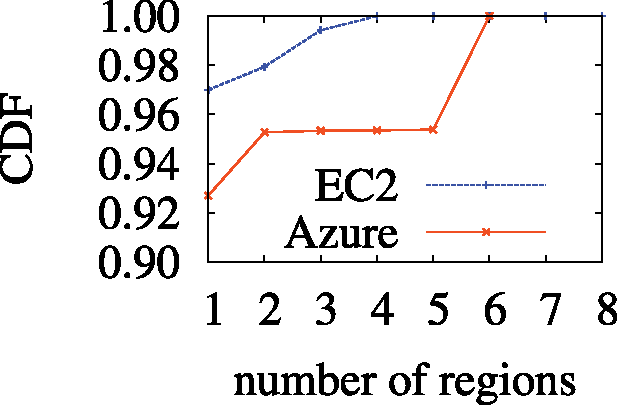
\includegraphics[width=\textwidth]{./figures/cloudmeasure/imag_sec4/region_cdf_new.pdf}
		\caption{subdomain}
		\label{fig:cloud_region_subdomains_CDF}
	\end{subfigure}
	\begin{subfigure}[b]{0.40\textwidth}
                \centering
                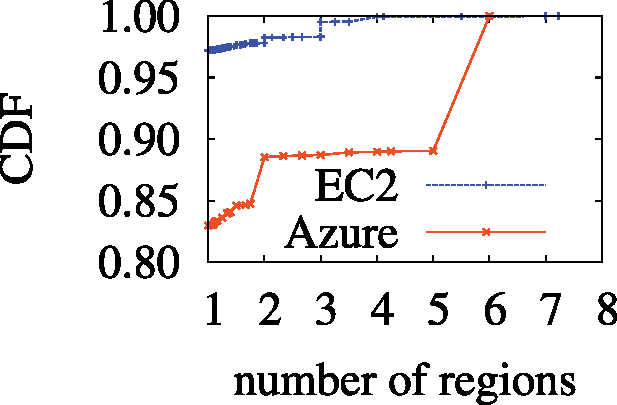
\includegraphics[width=\textwidth]{./figures/cloudmeasure/imag_sec4/region_cdf_new_avg.pdf}
		\caption{domain}
		\label{fig:cloud_region_domains_CDF}
	\end{subfigure}
\caption{(a) CDF of the number of regions used by each subdomain
(b) CDF of the average number of regions used by the subdomains of each domain.}
\label{fig:cloud_region_CDF}
\end{figure}


\begin{table}[t]
\centering
\small
\begin{tabular}{|c||c|c|c|c|c|c|} \hline
%{\bf Rank} & {\bf Domain} & {\bf \# Subdom} &  {\bf \# Regions} & {\bf
%    {\em k}=1}  & {\bf {\em k}=2} \\ \hline
& & {\bf \# Cloud} &  {\bf Total \#} & & \\ 
{\bf Rank} & {\bf Domain} & {\bf Subdom} &  {\bf Regions} & 
    {\bf {\em k}=1}  & {\bf {\em k}=2} \\ \hline
7   & live.com   &  18  & 3 & 18 &  0   \\ \hline
9      & amazon.com  & 2  & 1 & 2 &  0 \\ \hline %1,3,u
13      & linkedin.com  & 3  &  2 &  3   & 0 \\ \hline %1,u
18      & msn.com  & 89  & 5 & 78   & 11 \\ \hline
20      & bing.com  & 1  & 1 & 1   & 0 \\ \hline
29      & 163.com  & 4  & 1 & 4   & 0 \\ \hline
31      & microsoft.com  & 11  & 5 & 7   & 4 \\ \hline
35      & pinterest.com  & 18   & 1& 18 & 0 \\ \hline %u, 2
36      & fc2.com & 14  & 2 & 14   &  0  \\ \hline % 1,2,3
42      & ask.com  & 1  & 1 & 1   & 0 \\ \hline
47      & apple.com  & 1  & 1 & 1   & 0 \\ \hline
48     & imdb.com  & 2  & 1& 2  & 0   \\ \hline % 3
51      & hao123.com  & 1  & 1 & 1   & 0 \\ \hline
59     & go.com   & 4    & 1 & 4  &  0  \\\hline % n/a
\end{tabular}


%%%%%%%%%%%%%%%%%%%%%%%%%%%%%%%%%%%%%%%%
\iffalse
\begin{tabular}{|c||c|c|c|} \hline
Rank& domain & avg region count& avg zone count \\ \hline
9      & amazon.com  &  1.0 & 3.0\\ \hline %1,3,u
13      & linkedin.com  & 1.0 & 2.0\\ \hline %1,u
35      & pinterest.com     & 1.0 & 1.9\\ \hline %u, 2
36      & fc2.com & 1.0 & 1.9 \\ \hline % 1,2,3
48     & imdb.com  & 1.0 & 1.0  \\ \hline % 3
59     & go.com   & 1.0 & 1.3 \\\hline % n/a
75     & instagram.com  & 1.0 & 1.7 \\ \hline % 2, 3
86     & imgur.com  & 1.0 & 2.0 \\ \hline % 1, 3
92     & netflix.com  & 1.7 & 3.5\\ \hline % 4
119     & dropbox.com  &  1.0 & 1.0\\ \hline %n/a
\end{tabular}
\fi

\caption{Region usage for the top cloud-using domains. The third column 
is the number of cloud-using subdomains; fourth is the total number of 
regions used by a domain; and the $k=1$ and $k=2$ columns are the number of subdomains which
use one or two regions, respectively.}
\label{top_alexa_domains_deploy}
\end{table}



\tightparagraph{Analysis of top domains} We now focus on region usage of
subdomains corresponding to the most popular (according to Alexa
rankings) domains. Our analysis is summarized in
\tabref{top_alexa_domains_deploy}. As with the rest of our results
above, we see that in all but two cases, subdomains appear to use a
single region. The exceptions are msn.com and microsoft.com, where 11
of the 89 subdomains and 4 of 11 subdomains, respectively, use two
regions each. No popular subdomain uses three or more regions. We also
note that in some cases, a domain may deploy different subdomains
across different regions: e.g., live.com's 18 subdomains are spread
across 3 regions. Contrarily, there are domains whose subdomains 
are all deployed in one region (e.g., pinterest.com).

%\textcolor{red}{the following para is newly added!!!}


\tightparagraph{Analysis of subdomain deployment vs. customer location} An
interesting question about cloud service deployment is whether subdomains
are deployed near their customers? The answer to this question reveals whether
current cloud services are deployed in an ``optimal'' manner, because
deploying a service near customers usually leads to better client network 
performance (lower latency and higher throughput). 

To answer this question, we leverage the client geo-location information
provided by the Alexa web information service~\cite{alexawebinfo}.  For
example, at the time of writing, Alexa reported that 47\% of clients
accessing pinterest.com are from the United States, 10.4\% from India, 3.2\%
from the United Kingdom, 3.1\% from Canada, and 2.1\% from Brazil.  For each
domain, we define the ``customer country'' as the country where the largest
fraction of clients are located. We assume the customer country is the
same for all of a website's subdomains, as Alexa does not track subdomains
separately. For instance, the United States is the customer country for
pinterest.com (and its subdomains) based on our definition.

We performed the analysis for all of the cloud-using subdomains (about 713K)
in our dataset.  Our measurement methodology was able to successfully
identify approximately 538K (75\% of the total) subdomains' customer
country.  We find that 252K (47\%) subdomains' customer country is not the 
same as the country where this subdomain is hosted.  Moreover, 174K (32\%)
subdomains are not even hosted on the same continent as the subdomains'
customer country.  This implies that a large fraction of web services are 
probably not deployed in an optimal manner in terms of network performance.
We suspect that the current deployment posture is affected by 
computing, storage, and network costs and/or how long the cloud
region has existed. In \secref{cloud-measure-performance}, we explore how much
opportunity exists for improving wide-area performance through changes in
region usage.


\tightparagraph{Summary and implications} Our key finding in this section is
that most popular domains and subdomains appear to be using a single
region. This has significant implications on both the robustness and
performance of cloud-using web services. From an availability
perspective, an outage of EC2's {\em US East} region would take down critical
components of at least 2.3\% of the domains (61\% of EC2-using
domains) on Alexa's list of the top 1 million websites. This is a
lower bound, as our results do not include dependencies between
domains.  
From a performance perspective, our analysis of web service
deployment and customer locations reveals that a considerable fraction of
client traffic may travel farther than necessary due to suboptimal
provisioning.

